\documentclass{article}

% if you need to pass options to natbib, use, e.g.:
%     \PassOptionsToPackage{numbers, compress}{natbib}
% before loading neurips_2023

% ready for submission
\usepackage[final]{neurips_2023}

% to avoid loading the natbib package, add option nonatbib:
%    \usepackage[nonatbib]{neurips_2023}


\usepackage[utf8]{inputenc} % allow utf-8 input
\usepackage[T1]{fontenc}    % use 8-bit T1 fonts
\usepackage{hyperref}       % hyperlinks
\usepackage{url}            % simple URL typesetting
\usepackage{booktabs}       % professional-quality tables
\usepackage{amsfonts}       % blackboard math symbols
\usepackage{nicefrac}       % compact symbols for 1/2, etc.
\usepackage{microtype}      % microtypography
\usepackage{xcolor}         % colors

\usepackage{lipsum}         % placeholder text generation
\usepackage{subcaption} 
\usepackage{graphicx}



% Damit die (sub)sections wie in der angabe formatiert sind: 1.), ..., a.), ...
\renewcommand{\thesection}{\arabic{section}.)}
\renewcommand{\thesubsection}{\alph{subsection}.)}


\title{MLPC Report  - Task 2: Data Exploration}


% The \author macro works with any number of authors. There are two commands
% used to separate the names and addresses of multiple authors: \And and \AND.
%
% Using \And between authors leaves it to LaTeX to determine where to break the
% lines. Using \AND forces a line break at that point. So, if LaTeX puts 3 of 4
% authors names on the first line, and the last on the second line, try using
% \AND instead of \And before the third author name.


\author{% Sorry, musste die Namen alphabetisch anordnen, hätte mich sonst zu sehr getriggered :(
  Team OBSERVE \AND
  Johannes Grafinger 
  \And
  Jonas Gantar 
  \And 
  Leonhard Markus Spanring 
  \And 
  Reinhard Josef Pötscher
}

\begin{document}

\maketitle
\begin{contributions}
  \textcolor{blue}{Reinhard and Johannes (Group 1) were responsible for tasks 1.) Case Study and 2.) Annotation Quality} \\ 
  \textcolor{magenta}{Leonhard and Jonas (Group 2) were responsible for tasks 3.) Audio Features and 4.) Text Features of the report} \\ 
  \textcolor{red}{All of us together were responsible for task 5.) Conclusions} \\ 
  In the same constellation we created this report. We all worked on the presentation together, with Group 2 providing its content. We held regular meetings, where each group presented their results up to that point and the other critically reviewing their work.
\end{contributions}

\section{Case Study}
\label{sec:Case Study}

\subsection{}
\label{sec:Case Study:a}

\subsection{}
\label{sec:Case Study:b}

\subsection{}
\label{sec:Case Study:c}

\pagebreak

\section{Annotation Quality} 
\label{sec:Annotation Quality}


\subsection{How precise are the temporal annotations?}
\label{sec:Annotation Quality:a1}
Since we did not have any ground truth for when events occur within the files, we simply compared temporal differences of annotations from different annotators corresponding to the same region. A pair of annotations were said to correspond to the same region if both their respective onset and offset times separately do not deviate by more than 0.5 seconds. This of course introduces a trade-off between False Positives and False Negatives.
Then, the absolute differences in onset-/offset times and durations were gathered and plotted in histograms, shown in Figure ~\ref{fig:2_a}.

\begin{figure}[htbp]
  \centering
  \begin{subfigure}[b]{0.33\textwidth}
    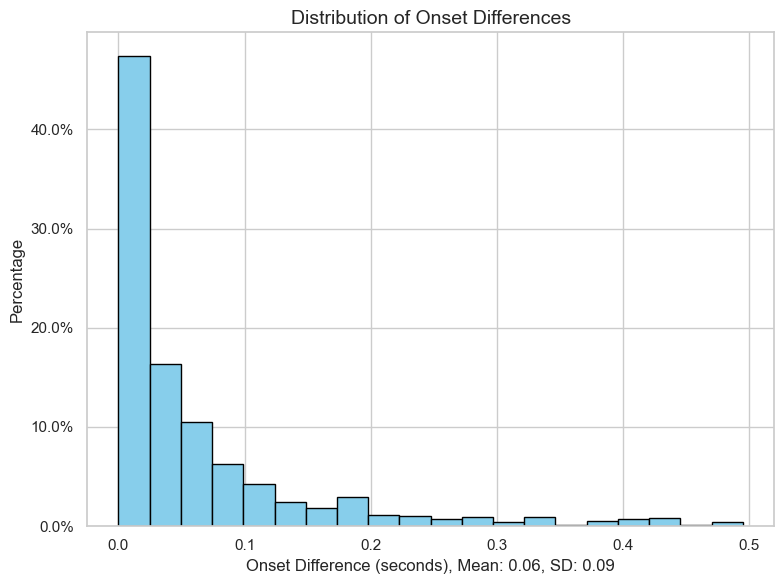
\includegraphics[width=\textwidth, height=4cm]{figs/onset_diffs.png}
  \end{subfigure}
  \hfill
  \begin{subfigure}[b]{0.33\textwidth}
    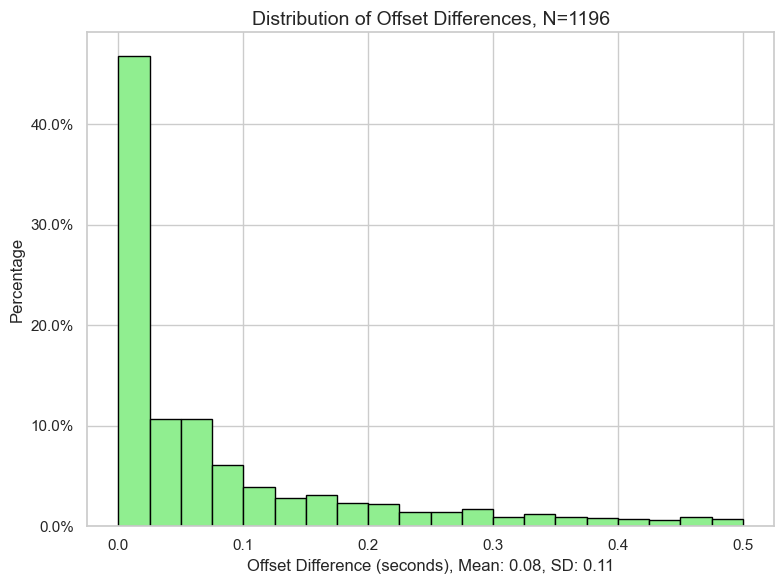
\includegraphics[width=\textwidth, height=4cm]{figs/offset_diffs.png}
  \end{subfigure}
  \hfill
  \begin{subfigure}[b]{0.33\textwidth}
    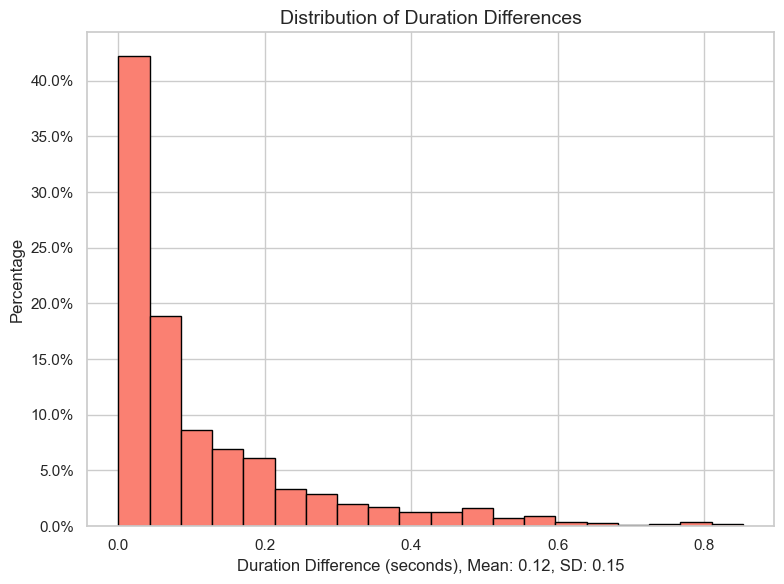
\includegraphics[width=\textwidth, height=4cm]{figs/duration_diffs.png}
  \end{subfigure}
  \caption{Absolute differences in onset-/offset times and durations for annotations corresponding to the same regions.}
  \label{fig:2_a}
\end{figure}

We can see that most annotations fall below a difference in onset-/offset times below 0.1 seconds. Depending on the temporal resolution of the audio features, this might actually lead to some falsely predicted frames in the future. Overall, most annotations seem to be pretty accurate.


\subsection{How similar are the text annotations that correspond to the same region?}
\label{sec:Annotation Quality:b1}
Using the same criterion as described above, we collected pairs of annotations corresponding to the same regions. For each of these pairs we then simply fetched their annotation text embeddings and calculated their cosine-similarity. The results can be seen in Figure ~\ref{fig:2_a}.

\begin{figure}[htbp]
  \centering
  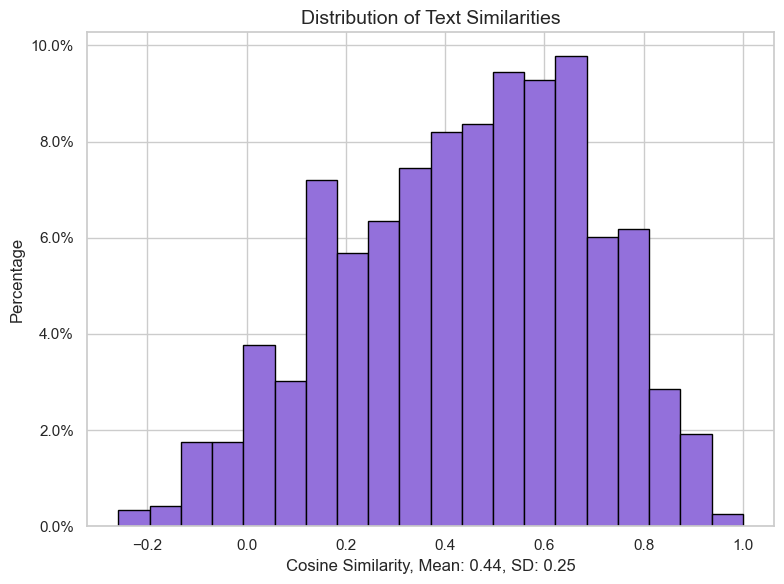
\includegraphics[width=0.5\textwidth, height=4cm]{figs/sim_diffs.png}
  \caption{Cosine similarities between annotations corresponding to the same regions.}
  \label{fig:2_b}
\end{figure}

We definitely see a similarity between the texts, as the bulk of the similarities lies above 0. We were a bit surprised that the average similarity is only 0.44, as we expected it to be way higher. We even found some similarities < 0, which might represent annotations containing some misinterpretations.

\subsection{How many annotations did we collect per file? How many distinct sound events per file?}
\label{sec:Annotation Quality:a2}
The number of annotations per file was easily calculated by grouping the corresponding dataframe by filenames.

Estimating the number of distinct sound events per file was a bit more complicated. For each set of annotations of one annotator for one file, we fetched the corresponding annotation embeddings and computed their pairwise cosine similarities. Say there $N$ annotations, they were then put into a $N \times N$ similarity matrix. This matrix was then filtered such that all values below a similarity threshold of 0.8 were set to 0 and all others to 1. This should give connected components within the graph corresponding to that matrix where the annotations are extremely similar, most likely because they describe the same sound event. Therefore the number of connected components is our estimate for the number of distinct sound events. If there were multiple annotators per file, the number was averaged and rounded. The results are shown in ~\ref{fig:2_c}.

\begin{figure}[htbp]
  \centering
  \begin{subfigure}[b]{0.49\textwidth}
    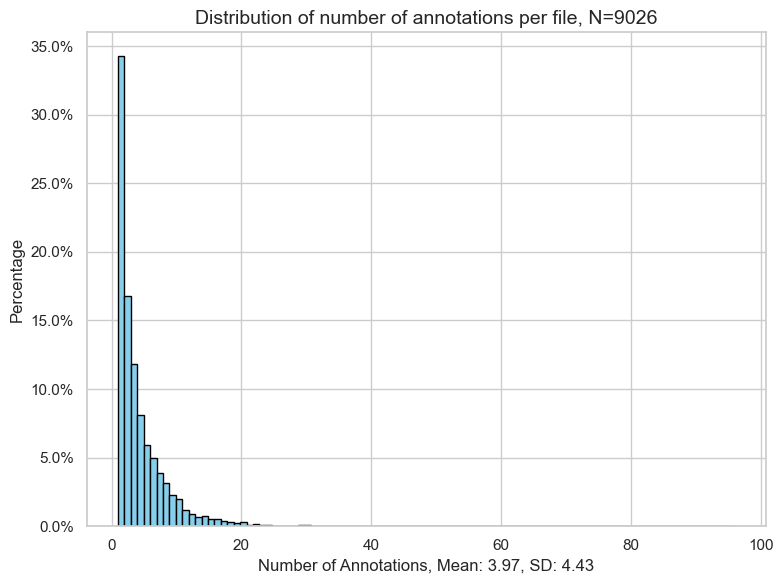
\includegraphics[width=\textwidth, height=4cm]{figs/annotation_dist.png}
  \end{subfigure}
  \hfill
  \begin{subfigure}[b]{0.49\textwidth}
    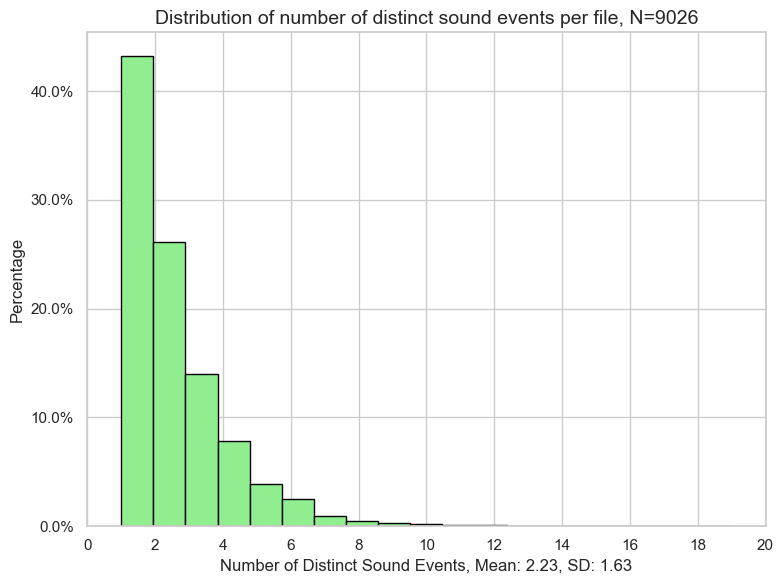
\includegraphics[width=\textwidth, height=4cm]{figs/sound_event_dist.png}
  \end{subfigure}
  \caption{Distributions of annotations and distinct sound events per file.}
  \label{fig:2_c}
\end{figure}

The results seem reasonable. We have an average of 3.97 annotations and 2.16 distinct sound events per file. Interestingly, the maximum number of annotations for a single file.

\subsection{How detailed are the text annotations? How much does the quality of annotations vary between
different annotators?}
\label{sec:Annotation Quality:b2}
As quality metrics for a single annotation,, we decided to compare the Text-Token-Ratio (TTR, number of unique word divided by the number of words), the number of spelling errors and the number of words. Analyzing the textual annotations for different annotators led us to the following ~\ref{fig:2_d}.

\begin{figure}[htbp]
  \centering
  \begin{subfigure}[b]{0.33\textwidth}
    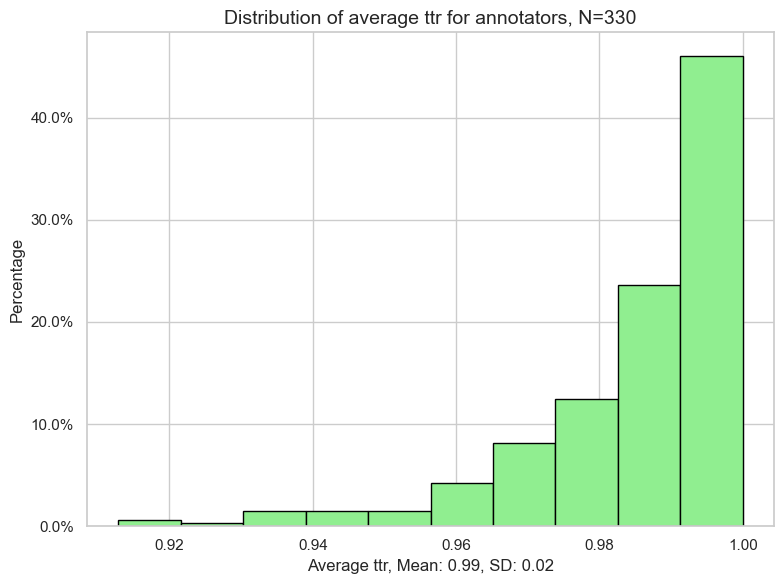
\includegraphics[width=\textwidth, height=4cm]{figs/ttr_dist.png}
  \end{subfigure}
  \hfill
  \begin{subfigure}[b]{0.33\textwidth}
    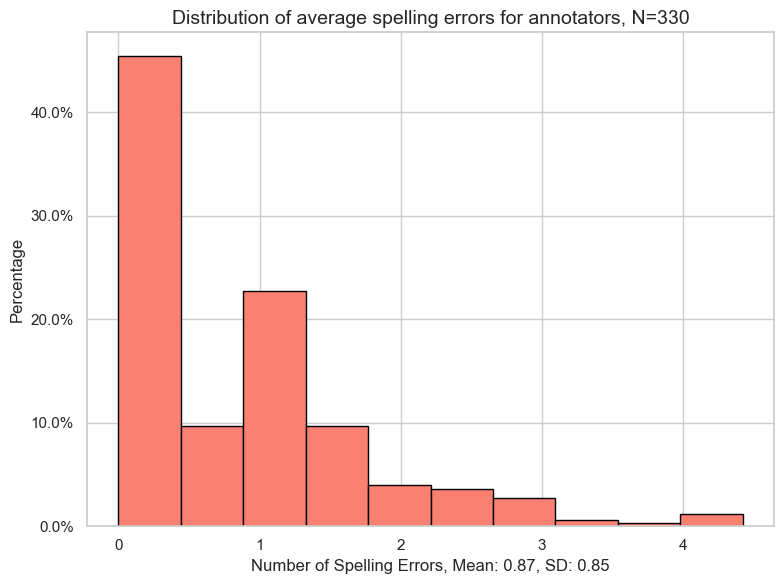
\includegraphics[width=\textwidth, height=4cm]{figs/error_dist.png}
  \end{subfigure}
  \hfill
  \begin{subfigure}[b]{0.33\textwidth}
    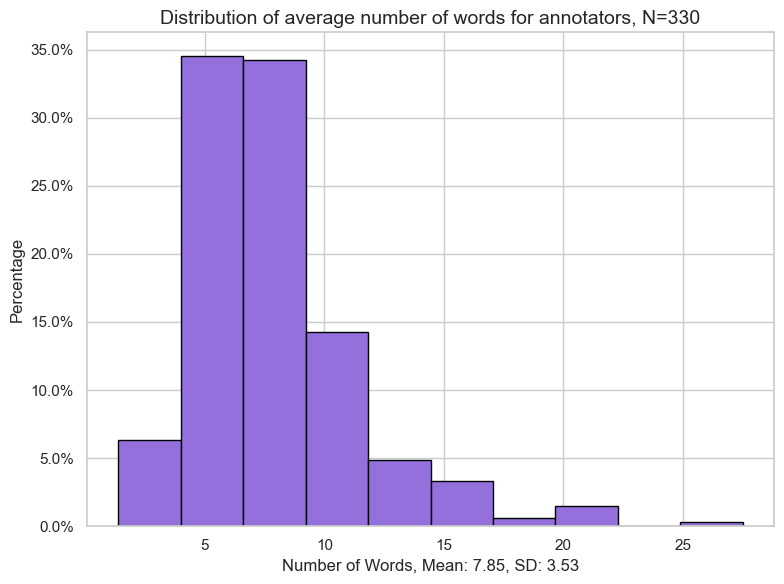
\includegraphics[width=\textwidth, height=4cm]{figs/word_dist.png}
  \end{subfigure}
  \caption{Distributions of quality metrics over all annotators.}
  \label{fig:2_d}
\end{figure}

The best metric out of these for checking how detailed the annotations are would most likely be the number of words per annotation. As the average annotator has written an average of 7.85 words per annotation, most of them seem to be reasonably detailed.
As for the variation in annotation quality: we were surprised to see that almost half of the annotators had on average more than 1 spelling error in their annotation. There also seem to be some with extremely low word counts. The standard deviation 3.53 for the average number of words seems reasonable as well. Most annotations should be of sufficient quality.
TTR turned out to be useless, as most annotations are so short that it would be very hard to find duplicate words.

\subsection{Are there any obvious inconsistencies, outliers, or poor-quality annotations in the data? Propose a
simple method to filter or fix incorrect or poor-quality annotations (e.g., remove outliers, typos, or
spelling errors).}
\label{sec:Annotation Quality:c2}
As our previous analysis has shown: yes, there are some poor quality annotations, i.e. outliers. This may be some consisting only of a single word or not relating to the audio because of some misconception. 
These could simply be removed by checking the word count of the annotations and removing the ones for which the text embedding is really dissimilar from metadata embeddings.
When it comes to fixing typos and spelling errors, one could simply use an off-the-shelf library (like in the above section) to go over the texts and correct them.


\pagebreak

\section{Audio Features}
\label{sec:Audio Features}

\subsection{}
\label{sec:Audio Features:a}

\subsection{}
\label{sec:Audio Features:b}

\subsection{}
\label{sec:Audio Features:c}




\section{Text Features}
\label{sec:Text Features}

\subsection{}
\label{sec:Text Features:a}

\subsection{}
\label{sec:Text Features:b}

\subsection{}
\label{sec:Text Features:c}




\section{Conclusions}
\label{sec:Conclusions}

\subsection{}
\label{sec:Conclusions:a}

\subsection{}
\label{sec:Conclusions:c}




% Put on a seperate page, just for referencing the guidelines
\pagebreak
\section{Submission of MLPC reports}

Please read the instructions below carefully and follow them faithfully. Note that this template is based on the official Neurips 2023 template. In your report, you may use three levels of headings, as described in what follows. 

\section{Headings: first level}
\label{sec:headings}

This is a first level heading. 

\subsection{Headings: second level}

This is a second level heading. 


\subsubsection{Headings: third level}

And this is a third level heading. Make sure to structure your report s.t. no deeper levels are necessary. 

\section{Footnotes, Figures and Tables}

\subsection{Footnotes}
Footnotes should be used sparingly. Note that footnotes are properly typeset \emph{after} punctuation marks.\footnote{As in this example.}


\subsection{Figures}


\begin{figure}
  \centering
  \fbox{\rule[-.5cm]{0cm}{4cm} \rule[-.5cm]{4cm}{0cm}}
  \caption{Sample figure caption.}
  \label{fig:example}
\end{figure}


All artwork must be neat, clean, and legible. Lines should be dark enough for
purposes of reproduction. You may use color figures. Please refer to all your figures in text, by using e.g., Figure~\ref{fig:example}. 

\subsection{Tables}
All tables must be centered, neat, clean and legible. Please refer to all your tables in text, by using e.g., Table~\ref{tab:example}.

Note that publication-quality tables \emph{do not contain vertical rules.} We
strongly suggest the use of the \verb+booktabs+ package.\footnote{\url{https://www.ctan.org/pkg/booktabs}}


\begin{table}
  \caption{Sample table title}
  \label{tab:example}
  \centering
  \begin{tabular}{lll}
    \toprule
    \multicolumn{2}{c}{Part}                   \\
    \cmidrule(r){1-2}
    Name     & Description     & Size ($\mu$m) \\
    \midrule
    Dendrite & Input terminal  & $\sim$100     \\
    Axon     & Output terminal & $\sim$10      \\
    Soma     & Cell body       & up to $10^6$  \\
    \bottomrule
  \end{tabular}
\end{table}


\section{Final instructions}

Do not change any aspects of the formatting parameters in the style files. In
particular, do not modify the width or length of the rectangle the text should
fit into, and do not change font sizes (this will result in a deduction of points). 
Please note that pages should be numbered, and adhere to the given \emph{page limit} to avoid further point deductions. Your final submission should be a \texttt{pdf} file.

%%%%%%%%%%%%%%%%%%%%%%%%%%%%%%%%%%%%%%%%%%%%%%%%%%%%%%%%%%%%


\end{document}